\subsection{Quadrat von Vektoren}
\subsubsection{Ziel der Multiplikation}
Was eine Addition von Vektoren bedeutet ist sehr intuitiv und auch leicht geometrisch darzustellen wie in Abbildung \ref{figure:addition}. Was allerdings das Produkt von Vektoren ergibt mag anfänglich unintuitiv wirken.
\begin{figure}[tb]
	\centering
		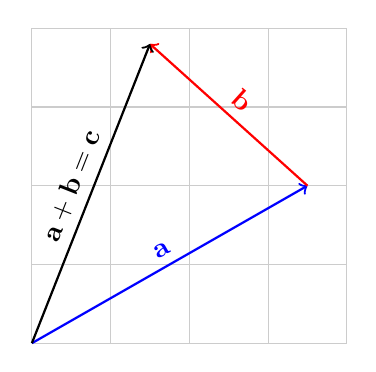
\begin{tikzpicture}
			\draw[thin,gray!40] (0,0) grid (4,4);
			\draw[blue,thick,->] (0,0)--(3.5,2) node[midway,above,sloped] {$\textbf{a}$};
			\draw[red,thick,->] (3.5,2)--(1.5,3.8) node[midway,above,sloped] {$\textbf{b}$};
			\draw[black,thick,->] (0,0)--(1.5,3.8)node[midway,above,sloped] {$\textbf{a} +\textbf{b} = \textbf{c} $};
		\end{tikzpicture}
		\caption{Addition von zwei Vektoren\label{figure:addition}}
\end{figure}
Was soll es schon heissen zwei Vektoren miteinander zu multiplizieren? 
Im Folgenden werden wir versuchen diese Operation ähnlich intuitiv darzustellen.

Um sinnvoll eine neue Operation zwischen zwei Elementen einer Algebra, in diesem Fall sind diese Elemente Vektoren, zu definieren, muss man überlegen, was das Ziel dieser Operation sein soll.
 
\begin{ziel}
	\label{clifford:ziel}
	Der Vektorraum der $n$-dimensionalen Vektoren soll zu einer Algebra so erweitert werden, dass das Quadrat von Vektoren durch die Länge des Vektors ausgedrückt werden kann.
\end{ziel}
Zusätzlich soll auch das Assoziativgesetz für die Multiplikation von Vektoren gelten, dass heisst wir dürfen wie in
\begin{equation}
    \label{eq:assoziativ}
    \textbf{e}_i(\textbf{e}_j + \textbf{e}_k) 
    = 
    \textbf{e}_i\textbf{e}_j + \textbf{e}_i\textbf{e}_k
\end{equation}
ausklammern.
Allerdings gilt das Kommutativgesetz leider, oder wie man sehen wird zum Glück, nur für skalare Elemente wie in
\begin{equation}
    \label{eq:kommSkalar}
    a\textbf{e}_ib\textbf{e}_j 
    = 
    ab\textbf{e}_i\textbf{e}_j \qquad a,b \in \mathbb{R}
\end{equation}
aber nicht für Vektoren. Im Allgemeinen wird
\begin{equation}
    \label{eq:kommVector}
    \textbf{e}_i\textbf{e}_j 
    \neq 
    \textbf{e}_j\textbf{e}_i
\end{equation}
sein.
\subsubsection{Quadrieren eines Vektors}
Betrachten wir nun mit diesen Regeln das Quadrat eines Vektors. Zuerst werden die Vektoren als Linearkombinationen geschrieben:
\begin{equation}
	    \textbf{a}^2 = 
		\left ( 
		\sum_{i=1}^{n} a_i \textbf{e}_i 
		\right ) 
		\left ( 
		\sum_{i=1}^{n} a_i \textbf{e}_i 
		\right )
		\label{eq:quad_a_1}.
\end{equation}
Das Quadrat kann nun in zwei Summen 
\begin{equation}
	\textbf{a}^2 =
	\textcolor{red}{\sum_{i=1}^{n} a_i^2\textbf{e}_i^2} 
	+ 
	\textcolor{blue}{\sum_{\begin{subarray}{l}i,j=1\\i \neq j\end{subarray}}^n  a_ia_j\textbf{e}_i\textbf{e}_j } 
	\label{eq:quad_a_2}
\end{equation}
aufgeteilt werden, wobei die roten Summe die quadrierten Terme und die blaue Summe die Mischterme beinhaltet.
Wie zuvor in \ref{clifford:ziel} definiert, ergibt das Quadrat eines Vektors dessen Länge. Da die Basisvektoren orthonormiert sind muss $\textbf{e}_i^2 = 1$ gelten.
\begin{equation}
	\textbf{a}^2 = \textcolor{red}{\sum_{i=1}^{n} a_i^2} + \textcolor{blue}{\sum_{\begin{subarray}{l}i,j=1\\i \neq j\end{subarray}}^n  a_ia_j\textbf{e}_i\textbf{e}_j}.
	\label{eq:quad_a_3}
\end{equation}
\begin{beispiel}
Das Quadrat des Vektor $\textbf{a}$ in $\mathbb{R}^2$ ist
\begin{equation}
    \begin{split}
    \textbf{a}^2 
    &= (a_1\textbf{e}_1+a_2\textbf{e}_2)(a_1\textbf{e}_1+a_2\textbf{e}_2) \\\
    &= \textcolor{red}{a_1^2\textbf{e}_1^2 + a_2^2\textbf{e}_2^2} 
    + \textcolor{blue}{a_1\textbf{e}_1a_2\textbf{e}_2 + a_2\textbf{e}_2a_1\textbf{e}_2}   \\\
    & = \textcolor{red}{a_1^2 + a_2^2} + \textcolor{blue}{a_1b\textbf{e}_1a_2\textbf{e}_2 + a_2\textbf{e}_2a_1\textbf{e}_2}.
    \end{split}
\end{equation}
\end{beispiel}

Der rote Teil von \ref{eq:quad_a_3} ist nun bereits die Länge im Quadrat, also das zuvor definierte Ziel der Multiplikation. 
Daraus lässt sich schliessen, dass der restliche Teil dieser Gleichung
\begin{equation}
    \label{eq:Mischterme_Null}
    \sum_{\begin{subarray}{l}i,j=1\\i \neq j\end{subarray}}^n  a_ia_j\textbf{e}_i\textbf{e}_j  = \textcolor{red}{a_1a_2(\textbf{e}_1\textbf{e}_2 + \textbf{e}_2\textbf{e}_1)} + a_1a_3(\textbf{e}_1\textbf{e}_3 + \textbf{e}_3\textbf{e}_1) + \dots =  0.
\end{equation}
 ergeben muss.
 Aus dieser Erkenntnis können weitere Eigenschaften für die Multiplikation hergeleitet werden.
 
Da dies für beliebige $a_i$ gelten muss werden alle Terme bis auf $a_1$ und $a_2$ gleich null gesetzt. Somit fallen alle Terme bis auf den roten weg. Wird dies weiter vereinfacht, ergibt sich
\begin{equation}
\begin{split}
    a_1a_2(\textbf{e}_1\textbf{e}_2 + \textbf{e}_2\textbf{e}_1) &= 0 \\
    a_1a_2\textbf{e}_1\textbf{e}_2 &= -a_1a_2\textbf{e}_2\textbf{e}_1 \\
    \textbf{e}_1\textbf{e}_2 &= -\textbf{e}_2\textbf{e}_1.
\end{split}
\end{equation}
\begin{satz}
  Die Multiplikation von orthogonalen Vektoren ist antikommutativ
    \begin{equation}
        \textbf{e}_i\textbf{e}_j = -\textbf{e}_j\textbf{e}_i \quad \textrm{für} \quad \textbf{e}_i \perp \textbf{e}_j.
    \end{equation}
\end{satz}
Dieses Wissen reicht nun bereits, um alle Produkte der Basisvektoren zu berechnen, was in Tabelle \ref{tab:multip_vec} gemacht wurde.
\begin{table}
\begin{center}
\begin{tabular}{ |c|ccccc| } 
 \hline
  & $\textbf{e}_1$ & $\textbf{e}_2$ & $\dots$ & $\textbf{e}_{n-1}$ & $\textbf{e}_{n}$ \\
  \hline
 $\textbf{e}_1$ & 1 & $\textbf{e}_1\textbf{e}_2$ & $\dots$ & $\textbf{e}_1\textbf{e}_{n-1}$ & $\textbf{e}_1\textbf{e}_{n}$ \\
 $\textbf{e}_2$ & $-\textbf{e}_1\textbf{e}_2$ & 1 & $\dots$ & $\textbf{e}_2\textbf{e}_{n-1}$ & $\textbf{e}_2\textbf{e}_{n}$ \\
 $\vdots$ & $\vdots$ & $\vdots$ & $\ddots$ & $\vdots$ & $\vdots$ \\
 $\textbf{e}_{n-1}$ & $-\textbf{e}_1\textbf{e}_{n-1}$ & $-\textbf{e}_2\textbf{e}_{n-1}$  & $\dots$ & $1$ & $\textbf{e}_{n-1}\textbf{e}_{n}$ \\
 $\textbf{e}_{n}$ & $-\textbf{e}_1\textbf{e}_{n}$ & $-\textbf{e}_2\textbf{e}_{n}$  & $\dots$ & $-\textbf{e}_{n-1}\textbf{e}_{n}$ & 1 \\
 \hline
\end{tabular}
\end{center}
\caption{Multiplikationstabelle für Vektoren}
\label{tab:multip_vec}
\end{table}
